
% Prepared by Calvin Kent
%
% Assignment Template v19.02
%
%%% 20xx0x/MATHxxx/Crowdmark/Ax
%
\documentclass[12pt]{article} %
\usepackage{amsthm}
\usepackage{CKpreamble}
\usepackage{CKassignment}
\usepackage{mdframed}
\usepackage{tikz}
\usepackage{pgfplots}

%
\begin{document}
	\pagenumbering{arabic}
	% Start of class settings ...
	\renewcommand*{\coursecode}{MATH 235} % renew course code
	\renewcommand*{\assgnnumber}{Assignment 1} % renew assignment number
	\renewcommand*{\submdate}{September 14, 2021} % renew the date
	\renewcommand*{\studentfname}{Abdullah} % Student first name
	\renewcommand*{\studentlname}{Zubair} % Student last name
    \renewcommand*{\proofname}{Proof:}
	% \renewcommand*{\studentnum}{20836288} % Student number

	\renewcommand\qedsymbol{$\blacksquare$}
	\setfigpath
	% End of class settings	
	% \pagestyle{crowdmark}
	\newgeometry{left=18mm, right=18mm, top=22mm, bottom=22mm} % page is set to default values
	\fancyhfoffset[L,O]{0pt} % header orientation fixed
	% End of class settings
	%%% Note to user:
	% CTRL + F <CHANGE ME:> (without the angular brackets) in CKpreamble to specify graphics paths accordingly.
	% The command \circled[]{} accepts one optional and one mandatory argument.
	% Optional argument is for the size of the circle and mandatory argument is for its contents.
	% \circled{A} produces circled A, with size drawn for letter A. \circled[TT]{A} produces circled A with size drawn for TT.
	% https://github.com/CalvinKent/My-LaTeX
	%%%

	%%%%%%%%%%%%%%%%%%%%%%%%%%%%%%%%%%%%%%%%%%%%%%%%%%%%%%%%%%%%%%%%%%%%%%%%%%%%%%%
	%%%                        CUSTOM MACRO VIM-TEX                             %%%
	%%       call IMAP('NOM', '\nomenclature{}', 'tex')               

	%%%%%%%%%%%%%%%%%%%%%%%%%%%%%%%%%%%%%%%%%%%%%%%%%%%%%%%%%%%%%%%%%%%%%%%%%%%%%%%

	% Crowdmark assignment start
	% qnumber, qname, qpoints

\begin{center}
	\textbf{\underline{\Huge{Lecture 2 - Homework}}}
\end{center}
\begin{qstn}
  Let $H = \{4,6,7,8,10,12,13,15\}$ and $T = \{1,2,5,7,8,10,12,14,16\}$. For each function described below, draw a
  mapping diagram between the two sets. Also state the range of the function.

  \begin{enumerate}[label=(\alph*)]
    \item 
         \begin{itemize}
            \item $f \colon \mathcal{H} \to \mathcal{T}$.
            \item \textbf{rule of $f$:} Take each element in $\mathcal{H}$, and subtract 2.
        \end{itemize}

    \item 
       \begin{itemize}
            \item $F \colon \mathcal{H} \to \mathcal{T}$.
            \item \textbf{rule of $F$:} Take each element in $\mathcal{H}$
              \begin{itemize}
                \item \textbf{IF} it is even, then divide it by 2
                \item \textbf{ELSE} if it is odd, then subtract $1$ first, then divide your result by $2$.
              \end{itemize}
        \end{itemize}
    \item
      \begin{itemize}
            \item $g \colon \mathcal{H} \to \mathcal{T}$.
            \item \textbf{rule of $g$:} Take each element in $\mathcal{H}$, and double it.
      \end{itemize}

    \item
      \begin{itemize}
            \item $I \colon \mathcal{H} \to \mathcal{T}$.
            \item \textbf{rule of $I$:} Take each element in $\mathcal{H}$, and multiply it by $1$.
            \item (This function is really important in advanced math! Specifically linear algebra, its called the identity
              function).
      \end{itemize}

  \end{enumerate}
\end{qstn}

\begin{qstn}
  Let $r \colon \mathcal{A} \to \mathcal{B}$ be a function that maps from $\mathcal{A}$ to $\mathcal{B}$. The figure below is the
  mapping diagram for $r$. Explain why $r$ cannot be a function. 

\begin{center}
 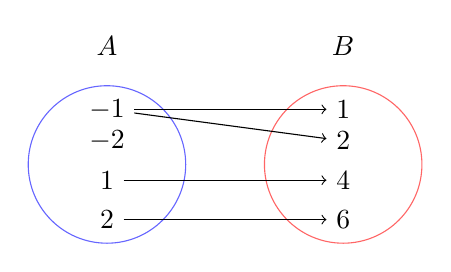
\begin{tikzpicture}
    % draw the sets
    \filldraw[fill=white!20, draw=blue!60] (-1.5,0) circle (1cm);
    \filldraw[fill=white!20, draw=red!60] (1.5,0) circle (1cm);


    % the texts
    \node at (-1.5,1.5) {$A$};
    \node at (1.5,1.5) {$B$};

    % the points in the sets (here I just create nodes to use them later on to position
    % the circles and the arrows
    \node (x1) at (-1.5,0.7) {$-1$};
    \node (x2) at (-1.5,0.3) {$-2$};
    \node (x3) at (-1.5,-0.2) {$1$};
    \node (x4) at (-1.5,-0.7) {$2$};
    \node (y1) at (1.5,0.7) {$1$};
    \node (y2) at (1.5,0.3) {$2$};
    \node (y3) at (1.5,-0.2) {$4$};
    \node (y4) at (1.5,-0.7) {$6$};

    % draw the arrows
    \draw[->] (x1) -- (y1);
    \draw[->] (x1) -- (y2);
    \draw[->] (x3) -- (y3);
    \draw[->] (x4) -- (y4);

\end{tikzpicture}
\end{center}

\end{qstn}


\begin{qstn}
	Translate the following symbolical rules to plain English.
		\begin{enumerate}[label=(\alph*)]
			\item \textbf{rule of $Q$:} For every element $a\in \mathcal{A}$, evaluate $Q(a) = 2a + 2$.
			\item \textbf{rule of $M$:} For every element $x\in \mathcal{X}$, evaluate $M(x) = \frac{x}{2} + 1$.
			\item \textbf{rule of $Z$:} For every element $b\in \mathcal{B}$, evaluate  $Z(b) = 3b$.
			\item \textbf{rule of $R$:} For every element $c\in \mathcal{C}$, evaluate $R(c) = -\sqrt{c} $.
			\item \textbf{rule of $S$:} For every element $y\in \mathcal{Y}$, evaluate $S(y) = y^2 + y^3$.
		\end{enumerate}
\end{qstn}

\begin{qstn}
  \textbf{Textbook, Pg 22:} Question 1
\end{qstn}

\newpage

\begin{qstn}
  Let $f(x) = 2x^2 - 5x + 3$ and $g(x) = 4x - 3$ be functions. Evaluate the following,
  \begin{enumerate}[label=(\alph*)]
    \item $f(0)$ \textbf{and} $g(0)$
    \item $f(3)$ \textbf{and} $g(-8)$
    \item $f(g(-8))$
    \item $g(f(-2))$
    \item $f(f(f(0)))$
  \end{enumerate}
  
\end{qstn}

\begin{qstn}
  Sketch the following functions. ALSO, state whether the vertex represents a maximum or a minimum.
  \begin{enumerate}[label=(\alph*)]
    \item $t(x) = -2x^2 + 4$
    \item $f(x) = x^2 - 7x + 12$
    \item $g(x) = -3x^2 + 7x - 6$
  \end{enumerate}
\end{qstn}




\end{document}




























